\documentclass[11pt]{article}

\usepackage[margin=1in]{geometry}
\usepackage{fancyhdr}
\usepackage{amsmath,amsfonts,amsthm,bm}
\usepackage{amssymb}
\pagestyle{fancy}


\usepackage[T1]{fontenc}
\usepackage{CJKutf8}

\CJKencfamily{UTF8}{bkai} % 使用標楷體


\AtBeginDocument{%
    \begin{CJK}{UTF8}{bkai}} % 使用標楷體
    \AtEndDocument{%
    \clearpage\end{CJK}}
    
\usepackage{pgfplots} % for histogram plotting

\pgfplotsset{
  compat=newest,
  xlabel near ticks,
  ylabel near ticks
}
    
\usepackage{pgf,tikz}
\usepackage{mathrsfs}
\usetikzlibrary{arrows}
\usetikzlibrary[patterns]
\usetikzlibrary{positioning}
\newdimen\nodeDist
\nodeDist=28mm

\setlength{\unitlength}{1pt}

\pgfdeclarepatternformonly[\GridSize]{MyGrid}{\pgfqpoint{-1pt}{-1pt}}{\pgfqpoint{4pt}{4pt}}{\pgfqpoint{\GridSize}{\GridSize}}%
{
  \pgfsetlinewidth{0.3pt}
  \pgfpathmoveto{\pgfqpoint{0pt}{0pt}}
  \pgfpathlineto{\pgfqpoint{0pt}{3.1pt}}
  \pgfpathmoveto{\pgfqpoint{0pt}{0pt}}
  \pgfpathlineto{\pgfqpoint{3.1pt}{0pt}}
  \pgfusepath{stroke}
}

\pgfdeclarepatternformonly[\GridSize]{MyGrid2}{\pgfqpoint{-1pt}{-1pt}}{\pgfqpoint{4pt}{4pt}}{\pgfqpoint{\GridSize}{\GridSize}}%
{
  \pgfsetlinewidth{0.3pt}
  \pgfpathmoveto{\pgfqpoint{0pt}{0pt}}
  \pgfpathlineto{\pgfqpoint{0pt}{-30pt}}
  \pgfpathmoveto{\pgfqpoint{0pt}{0pt}}
  \pgfpathlineto{\pgfqpoint{-30pt}{0pt}}
  \pgfusepath{stroke}
}

\newdimen\GridSize
\tikzset{
    GridSize/.code={\GridSize=#1},
    GridSize=3pt
}



\definecolor{qqqqff}{rgb}{0.,0.,1.}
\definecolor{ffqqqq}{rgb}{1.,0.,0.}
\definecolor{qqwuqq}{rgb}{0.,0.39215686274509803,0.}
\definecolor{cqcqcq}{rgb}{0.7529411764705882,0.7529411764705882,0.7529411764705882}

\usepackage{enumitem}
\usepackage{fancybox}
\usepackage{sectsty}
\allsectionsfont{\centering}
\PassOptionsToPackage{hyphens}{url}\usepackage[colorlinks=true, urlcolor=black, hyperfootnotes=false]{hyperref}

\lhead{Machine Learning Techniques (NTU, Spring 2017)}
\chead{}
\rhead{王冠鈞(b03902027)}



\begin{document}


\section*{Homework \#4}
\subsection*{Answer Sheet}
\begin{center}
DEADLINE: 06/20/2017, 14:00\\
INSTRUCTOR:  Hsuan-Tien Lin\\[0.5cm]
王冠鈞 b03902027
\end{center}


\begin{enumerate}[label=\textbf{\arabic*}.]
	\item The probability that an example $\mathbf{x}_i$ is not sampled from bootstrapping is: 
  \[P(\mathbf{x}_i \text{ is not sampled}) = \left(\frac{N-1}{N}\right)^{N'}\]
      When $N$ is large, it is equivalent to\footnote{Since $\exp(x) = \lim_{n\rightarrow \infty} \left(1+\frac{x}{n}\right)^n$}:
      \[\lim_{N \rightarrow \infty} \left(\frac{N-1}{N}\right)^{N'} = \left(\lim_{N \rightarrow \infty} \left(1 + \frac{-1}{N}\right)^{N}\right)^p = e^{-p}\]
      Thus the (expected) number of examples that are not sampled is $N\cdot e^{-p}$.

  \item Since $G = \text{Uniform}(\{g_t\})$, for any example, there must be more than a half of trees that will mis-classify it to contribute to an error of $G$. In this question, there are 3 trees, so an example will contribute to $E_\text{out}(G)$ if and only if there are at least 2 trees make mistake on it. Thus, the lowest $E_\text{out} = 0$, when all mistakes from $g_1, g_2, g_3$ are disjointed (and it's possible to perfectly disjoint since $\sum_{i=1}^3 E_\text{out}(g_i) = 0.75 < 1$). That is, define $E_\text{out}^k = \{\textbf{x}_i | [\![ y_i \neq g_k(\textbf{x}_i)  ]\!] \}, k = 1, 2, 3$ and $E_\text{out}^G = \{\textbf{x}_i | [\![ y_i \neq G(\textbf{x}_i)  ]\!] \}$, then for any $i, j (1\leq i, j \leq 3, i \neq j)$, $E_\text{out}^i \cap E_\text{out}^j = \emptyset \Leftrightarrow E_\text{out}^G = \emptyset \Leftrightarrow E_\text{out}(G) = 0$. Oppositely, the maximum $E_\text{out}(G)$ occurs when all error examples are in exactly two of the three $E_\text{out}^k$. This will lead to the upper bound of $E_\text{out}(G) = \frac{1}{2}(0.15+0.25+0.35) = 0.375$. Combine the results together, we get the range of $E_\text{out}(G)$:
  \[0 \leq E_\text{out}(G) \leq 0.375 \]

  \item Reusing the definition and the concept in the previous question, if an example $\mathbf{x}_i \in E_\text{out}^G$, then there must be at least $\frac{K+1}{2}$ (more than a half) different $k$ such that $\mathbf{x}_i \in E_\text{out}^k$. Thus the upper bound of $E_\text{out}$ is \[E_\text{out} (G) \leq \frac{\sum_{k=1}^K e_k}{\frac{K+1}{2}} = \frac{2}{K+1} \sum_{k=1}^K e_k\]
  , in this case $\forall \mathbf{x}_i \in E_\text{out}^G$, there exist exactly $\frac{K+1}{2}$ trees that make mistake on $\mathbf{x}_i$.

  \item The new $s_n$, say it $s_n^{(1)}$, is updated from old $s_n$, say it $s_n^{(0)}$. According to the algorithm, we know that $s_n \leftarrow s_n + \alpha_1 g_1(\mathbf{x}_n)$. The new $s_n (s_n^{(1)})$ is derived as the following:
  \[\begin{aligned} s_n^{(1)} &= s_n^{(0)} + \alpha_1 g_1(\mathbf{x}_n)\\
  &= 0 + \text{OneVarLinearRegression}(\{(g_t(\mathbf{x}_n), y_n - 0)\})\\
  &= \frac{\sum_{n=1}^N g_1(\mathbf{x}_n)(y_n-s_n)}{\sum_{n=1}^N g_1^2 (\mathbf{x_n})}\cdot g_1(\mathbf{x}_n)\\
  &= \frac{\sum_{n=1}^N 2(y_n-0)}{\sum_{n=1}^N 4}\cdot 2 \\
  &= \frac{\sum_{n=1}^N 2y_n}{4N}\cdot 2 \\ 
  &= \frac{1}{N}\sum_{n=1}^N y_n\end{aligned}\]

  \item The value $\alpha_t$ can be represented as a closed-form formula:
  \[\alpha_t = \eta^* = \frac{\sum_{n=1}^N g_t(\mathbf{x}_n)(y_n-s_n^{(t-1)})}{\sum_{n=1}^N g_t^2 (\mathbf{x}_n)}\], where $s_n^{(t-1)}$ is the value of $s_n$ in the $(t-1)$-th iteration. We can arrange it into the following:
  \[\begin{aligned}&\alpha_t \cdot \sum_{n=1}^N g_t^2 (\mathbf{x}_n) = \sum_{n=1}^N g_t(\mathbf{x}_n)y_n - \sum_{n=1}^N g_t(\mathbf{x}_n)s_n^{(t-1)} \\ 
  \overset{\text{\phantom{asasasasdasdasdasdaasd}}}{\Rightarrow} & \sum_{n=1}^N g_t(\mathbf{x}_n)\cdot (s_n^{(t-1)} + \alpha_t g_t(\mathbf{x}_n)) = \sum_{n=1}^N g_t(\mathbf{x}_n)y_n \\
  \overset{\because s_n^{(t)} = s_n^{(t-1)} + \alpha_t g_t(\mathbf{x}_n)}{\Rightarrow} & \sum_{n=1}^N g_t(\mathbf{x}_n)\cdot s_n^{(t)} = \sum_{n=1}^N g_t(\mathbf{x}_n)y_n\end{aligned}\]
  And we directly get $\sum_{n=1}^N s_n g_t (\mathbf{x}_n) = \sum_{n=1}^N y_n g_t(\mathbf{x}_n)$ from above.

  \item \begin{proof}In the first step in the 1st iteration ($s_n = 0$), we have found a $g_1$ such that $\frac{1}{N} \sum_{n=1}^N (y_n - g_1(\mathbf{x}_n))^2$ (squared error of linear regression) is the smallest. In the second step, the algorithm will solve the following optimization problem:
  \[\underset{\alpha_1}{\min}\ \ \frac{1}{N} \sum_{n=1}^N ((y_n-0) -\alpha_1 g_1(\mathbf{x}_n))^2\]

  Note that this optimization problem has the same form of the previous step, and we have known that $g_1$ is the optimal function for the first step. In other words, we can use the result from the first step to directly solve this problem, and the optimal condition is:
  \[g_1(\mathbf{x}_n) = \alpha_1 g_1(\mathbf{x}_n)\]
  The condition holds only when $\alpha_1 = 1$. Thus the statement holds.

  \end{proof}

  \item \begin{proof}From question 6, we get $\alpha_1 = 1$. Then the new $s_n = s_n^{(1)} = s_n^{(0)} + 1\cdot g_1(\mathbf{x}_n) = g_1(\mathbf{x}_n)$. Since $g_1$ is derived from linear regression, after recalling from the Lecture 9 of ML Foundations\footnote{\url{http://www.csie.ntu.edu.tw/~htlin/mooc/doc/09_handout.pdf\#12}, the linear regression algorithm}, $g_1(\mathbf{x}_n) = (X^\dag\mathbf{y})^T\mathbf{x}_n$, where the symbols are defined in the linear regression lecture.\par
  Now in the 2nd iteration, the algorithm will find $g_2$, which is the optimal solution of \\ $\text{LinearRegression}(\{(\mathbf{x}_n), y_n - g_1(\mathbf{x}_n)\})$. According to the linear algorithm in MLF Lecture 9, the solution can be derived below:
  \[\begin{aligned}g_2(\mathbf{x}_n) = (\mathbf{w}_{\mathsf{LIN}}^{(2)})^T\mathbf{x}_n &= \left(X^\dag (\mathbf{y} - g_1(\mathbf{x}))\right)^T \mathbf{x}_n \\
   &= \left(X^\dag (\mathbf{y} - ((X^\dag\mathbf{y})^T X^T)^T )\right)^T \mathbf{x}_n \\
   &= \left(X^\dag (\mathbf{y} - XX^\dag\mathbf{y}) \right)^T \mathbf{x}_n \\
   &= \left((X^TX)^{-1}X^T (\mathbf{y} - X(X^TX)^{-1}X^T\mathbf{y}) \right)^T \mathbf{x}_n \\
   &= \left((X^TX)^{-1}X^T \mathbf{y} - (X^TX)^{-1}(X^T X)(X^TX)^{-1}X^T\mathbf{y} \right)^T \mathbf{x}_n \\
   &= \left((X^TX)^{-1}X^T \mathbf{y} - (X^TX)^{-1}X^T\mathbf{y} \right)^T \mathbf{x}_n \\
   &= \mathbf{0}^T\cdot \mathbf{x}_n \\
   &= 0
   \end{aligned}\]
   Thus the statement holds.

  \end{proof}

  \item The \texttt{OR} operation means that any of $x_1, x_2, \cdots, x_d$ is TRUE returns TRUE, i.e. only when all $x_i$ are FALSE will make $\sum_{i=0}^d w_i x_i < 0$. To achieve that, we can set $w_0 = d-1$ and $w_i = +1 (i \in 1, 2, \cdots , d)$, (i.e. $(w_0, w_1, w_2, \cdots, w_d) = (d-1, +1, +1, \cdots, +1)$) such that only when $x_1=x_2=\cdots = x_d = -1$ will make $\sum_{i=0}^d w_i x_i = -1 < 0$.

  \item The \texttt{XOR} operation has the property: $\mathtt{XOR}(x_1, x_2, x_3) = \mathtt{XOR}(\mathtt{XOR}(x_1, x_2),x_3)$. In this question, there are 5 inputs, and the \texttt{XOR} operation will return TRUE when there are exactly odd number of $+1$, and will return FALSE otherwise. The least number to implement a 5-input \texttt{XOR}, in my opinion is $D = 5$. To implement such a 5-5-1 NNet, we can define the meaning the nodes in the middle layer of the neuron net: \textit{the i-th (except the 0-th, which is always $+1$) node in the middle layer denotes that whether there are at least $(6-i)$ inputs with value $= +1$.} With such definition, the weight of the first layer can be defined:
  \[\begin{aligned}w_{i1}^{(1)} = (-5, +1, +1, +1, +1, +1) \\
  w_{i2}^{(1)} = (-4, +1, +1, +1, +1, +1) \\
  w_{i3}^{(1)} = (-3, +1, +1, +1, +1, +1) \\
  w_{i4}^{(1)} = (-2, +1, +1, +1, +1, +1) \\
  w_{i5}^{(1)} = (-1, +1, +1, +1, +1, +1)  \end{aligned}\]
  , and the second layer:
  \[w_{i1}^{(2)} = (-1, +1, -1, +1, -1, +1)\]

  If there are odd (even) number of positive inputs, then the second layer will make it become positive and return TRUE (FALSE).

  \item We already know: \[\begin{aligned} &\frac{\partial e_n}{\partial w_{ij}^{(l)}} &=\ & \delta_j^{(l)}\cdot \left(
  x_i^{(l-1)}\right) &\\ \text{where } & \delta_j^{l} &=\ & -2\left(y_n - s_1^{(L)}\right) & \text{ if }&l = L \\& \delta_j^{l} &=\ & \sum_k \left(\delta_k^{(l+1)}\right) \left(w_{jk}^{(l+1)}\right) \left(\tanh \left(s_j^{(l)}\right)\right) & \text{ if }&1 \leq l < L\end{aligned}\]
  And from this problem, all initial weights $w_{ij}^{l}$ are 0, which will make the term\\ $\sum_k \left(\delta_k^{(l+1)}\right) \left(w_{jk}^{(l+1)}\right) \left(\tanh \left(s_j^{(l)}\right)\right) = \sum_k \left(\delta_k^{(l+1)}\right) \left(0\right) \left(\tanh \left(s_j^{(l)}\right)\right) =  0$. That is, for $1 \leq l < L,\delta_j^{(l)} = 0 \Rightarrow \frac{\partial e_n}{\partial w_{ij}^{(l)}} = 0 \cdot \left(x_i^{(l-1)}\right)=0$.\par

  Now that we know when $1\leq l < L$, the all the gradient components $\frac{\partial e_n}{\partial w_{ij}^{(l)}} = 0$. We now examine what will lead to when $l = L$. We know that $\frac{\partial e_n}{\partial w_{ij}^{(L)}} = -2\left(y_n - s_1^{(L)}\right)\cdot\left(x_i^{(L-1)}\right)$, which has no weights that will directly lead it to 0. However, note that the term $\left(x_i^{(L-1)}\right)$ here, which denotes the hyperbolic tangent of the score to the neurons in the previous layer, and since \[\text{for } i \neq 0, x_i^{(L-1)} = \tanh (s_i^{(L-1)}) = \tanh (\sum_{j=0}^{d^{(L-2)}}w_{ji}^{(L-1)}x_j^{(L-2)}) = \tanh(0) = 0\]
  , which are also 0. However, note that when $i = 0$, $x_i^{(L-1)} = +1$ (according to the neural network model), and $\frac{\partial e_n}{\partial w_{01}^{(L)}} = -2\left(y_n - s_1^{(L)}\right)$, which is not necessarily 0 (depend on $[\![ y_n = s_1^{(L)} ]\!]$). For all the others, $\frac{\partial e_n}{\partial w_{ij}^{(l)}} = 0$.

  \item \begin{proof} 
    In the first step (stochastic), it just alter the input $\mathbf{x}$, and is nothing to do with the proof here.\par
    In the second step (forward), it will compute all $x_j^{(1)} = \tanh \left(\sum_{i=1}^{d^{(0)}}w_{ij}^{(1)}x_i^{(0)}\right)$. Since all $w_{ij}^{(1)}$ now is $1$, it's apparent that $x_1^{(1)} = x_2^{(1)} = \cdots = x_{d^{(1)}}^{(1)} \neq x_0^{(1)} = +1$. \par
    In the third step (backward), it will perform backpropagation and compute $\delta_j^{(l)}$. it will first compute $\delta_1^{(2)} = -2 \left(y_n - \sum_{i=1}^{d^{(1)}}w_{i1}^{(2)}x_i^{(1)} \right)$. Then it will compute $\delta_i^{(1)} = \left(\delta_1^{(2)}\right)\left(w_{i1}^{(2)}\right) \left(\tanh'\left(s_i^{(1)}\right)\right)$. We know that $\delta_1^{(2)}$ is fixed here, as shown above, and all $w_{i1}^{(2)} = 1$, and we further notice that since $s_i^{(1)} = \sum_{i=1}^{d^{(0)}}w_{ij}^{(1)}x_i^{(0)}$, with the same reason of the previous step, we get $s_1^{(1)} = \cdots = s_{d^{(1)}}^{(1)}$ and thus $\delta_1^{(1)} = \delta_2^{(1)} = \cdots = \delta_{d^{(1)}}^{(1)}$. \par 
    In the fourth step (gradient descent), it will perform $w_{ij}^{(1)} \leftarrow w_{ij}^{(1)} - \eta x_i^{(0)}\delta_j^{(1)}$. For $0 \leq i \leq d^{(0)}$ and for $1 \leq j < d^{(1)}$, we have initially $w_{ij}^{(1)}=w_{i(j+1)}^{(1)}=1$ and from the previous step we have $\delta_j^{(1)} = \delta_{(j+1)}^{(1)}$. Thus after gradient descent, we have the new $w_{ij}^{(1)} = 1 - \eta x_i^{(0)}\delta_j^{(1)} = 1 - \eta x_i^{(0)}\delta_{(j+1)}^{(1)} = w_{i(j+1)}^{(1)}$. Thus the statement holds.

  \end{proof}

  \item Here is the histogram, where the x axis is $E_\text{in}(g_t)$, and the y axis denotes the number of trees that lead to such $E_\text{in}$.\\
  \begin{picture}(0,0)
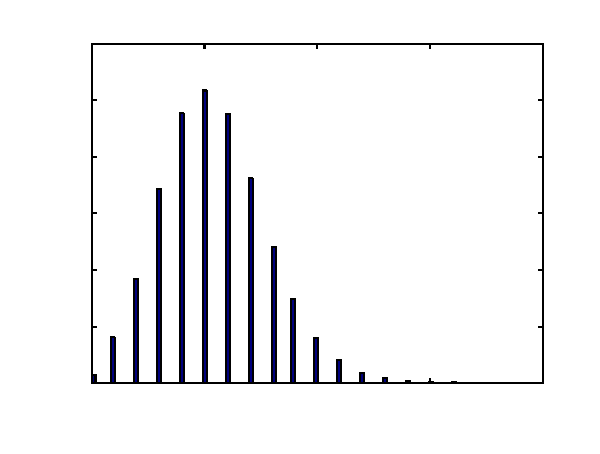
\includegraphics{plot/q12-inc}
\end{picture}%
\begin{picture}(288,218)(0,0)
\fontsize{10}{0}
\selectfont\put(44.0044,28.9956){\makebox(0,0)[t]{\textcolor[rgb]{0,0,0}{{0}}}}
\fontsize{10}{0}
\selectfont\put(98.1636,28.9956){\makebox(0,0)[t]{\textcolor[rgb]{0,0,0}{{0.05}}}}
\fontsize{10}{0}
\selectfont\put(152.322,28.9956){\makebox(0,0)[t]{\textcolor[rgb]{0,0,0}{{0.1}}}}
\fontsize{10}{0}
\selectfont\put(206.481,28.9956){\makebox(0,0)[t]{\textcolor[rgb]{0,0,0}{{0.15}}}}
\fontsize{10}{0}
\selectfont\put(260.64,28.9956){\makebox(0,0)[t]{\textcolor[rgb]{0,0,0}{{0.2}}}}
\fontsize{10}{0}
\selectfont\put(39.0127,33.9961){\makebox(0,0)[r]{\textcolor[rgb]{0,0,0}{{0}}}}
\fontsize{10}{0}
\selectfont\put(39.0127,61.1631){\makebox(0,0)[r]{\textcolor[rgb]{0,0,0}{{1000}}}}
\fontsize{10}{0}
\selectfont\put(39.0127,88.3306){\makebox(0,0)[r]{\textcolor[rgb]{0,0,0}{{2000}}}}
\fontsize{10}{0}
\selectfont\put(39.0127,115.498){\makebox(0,0)[r]{\textcolor[rgb]{0,0,0}{{3000}}}}
\fontsize{10}{0}
\selectfont\put(39.0127,142.666){\makebox(0,0)[r]{\textcolor[rgb]{0,0,0}{{4000}}}}
\fontsize{10}{0}
\selectfont\put(39.0127,169.833){\makebox(0,0)[r]{\textcolor[rgb]{0,0,0}{{5000}}}}
\fontsize{10}{0}
\selectfont\put(39.0127,197){\makebox(0,0)[r]{\textcolor[rgb]{0,0,0}{{6000}}}}
\fontsize{10}{0}
\selectfont\put(152.322,17.9956){\makebox(0,0)[t]{\textcolor[rgb]{0,0,0}{{$E_{in}(g_t)$}}}}
\fontsize{10}{0}
\selectfont\put(11.0127,115.498){\rotatebox{90}{\makebox(0,0)[b]{\textcolor[rgb]{0,0,0}{{number of trees}}}}}
\fontsize{10}{0}
\selectfont\put(152.322,207){\makebox(0,0)[b]{\textcolor[rgb]{0,0,0}{{Result of Question 12}}}}
\end{picture}


  \item The relation between $t$ and $E_\text{in}(G_t)$ is shown below. \\
  \setlength{\unitlength}{1pt}
\begin{picture}(0,0)
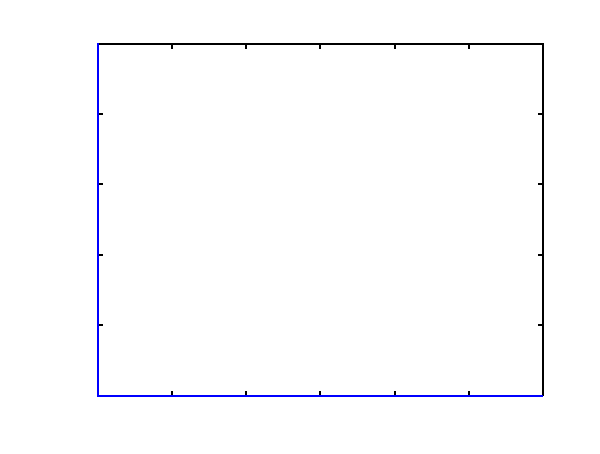
\includegraphics{plot/q13-inc}
\end{picture}%
\begin{picture}(288,218)(0,0)
\fontsize{10}{0}
\selectfont\put(47.0044,22.9956){\makebox(0,0)[t]{\textcolor[rgb]{0,0,0}{{0}}}}
\fontsize{10}{0}
\selectfont\put(82.6104,22.9956){\makebox(0,0)[t]{\textcolor[rgb]{0,0,0}{{5000}}}}
\fontsize{10}{0}
\selectfont\put(118.216,22.9956){\makebox(0,0)[t]{\textcolor[rgb]{0,0,0}{{10000}}}}
\fontsize{10}{0}
\selectfont\put(153.822,22.9956){\makebox(0,0)[t]{\textcolor[rgb]{0,0,0}{{15000}}}}
\fontsize{10}{0}
\selectfont\put(189.428,22.9956){\makebox(0,0)[t]{\textcolor[rgb]{0,0,0}{{20000}}}}
\fontsize{10}{0}
\selectfont\put(225.034,22.9956){\makebox(0,0)[t]{\textcolor[rgb]{0,0,0}{{25000}}}}
\fontsize{10}{0}
\selectfont\put(260.64,22.9956){\makebox(0,0)[t]{\textcolor[rgb]{0,0,0}{{30000}}}}
\fontsize{10}{0}
\selectfont\put(42.0132,27.9961){\makebox(0,0)[r]{\textcolor[rgb]{0,0,0}{{0}}}}
\fontsize{10}{0}
\selectfont\put(42.0132,61.7969){\makebox(0,0)[r]{\textcolor[rgb]{0,0,0}{{0.01}}}}
\fontsize{10}{0}
\selectfont\put(42.0132,95.5977){\makebox(0,0)[r]{\textcolor[rgb]{0,0,0}{{0.02}}}}
\fontsize{10}{0}
\selectfont\put(42.0132,129.398){\makebox(0,0)[r]{\textcolor[rgb]{0,0,0}{{0.03}}}}
\fontsize{10}{0}
\selectfont\put(42.0132,163.199){\makebox(0,0)[r]{\textcolor[rgb]{0,0,0}{{0.04}}}}
\fontsize{10}{0}
\selectfont\put(42.0132,197){\makebox(0,0)[r]{\textcolor[rgb]{0,0,0}{{0.05}}}}
\fontsize{10}{0}
\selectfont\put(153.822,11.9956){\makebox(0,0)[t]{\textcolor[rgb]{0,0,0}{{t}}}}
\fontsize{10}{0}
\selectfont\put(17.0132,112.498){\rotatebox{90}{\makebox(0,0)[b]{\textcolor[rgb]{0,0,0}{{$E_{in}(G_t)$}}}}}
\fontsize{10}{0}
\selectfont\put(153.822,207){\makebox(0,0)[b]{\textcolor[rgb]{0,0,0}{{Result of Question 13}}}}
\end{picture}

  \item The relation between $t$ and $E_\text{out}(G_t)$ is shown below. As we can see, when $t$ is large, both $E_\text{in}$ and $E_\text{out}$ will end up being constant. The difference is that the terminal $E_\text{in}$ is zero, while the terminal $E_\text{out}$ is 0.071.\\
  \begin{picture}(0,0)
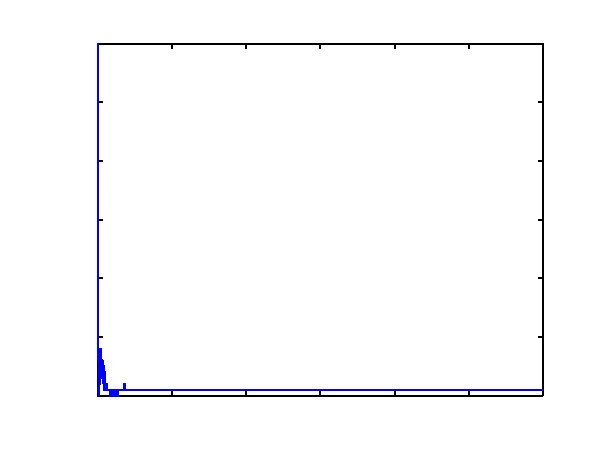
\includegraphics{plot/q14-inc}
\end{picture}%
\begin{picture}(288,218)(0,0)
\fontsize{10}{0}
\selectfont\put(47.0044,22.9956){\makebox(0,0)[t]{\textcolor[rgb]{0,0,0}{{0}}}}
\fontsize{10}{0}
\selectfont\put(82.6104,22.9956){\makebox(0,0)[t]{\textcolor[rgb]{0,0,0}{{5000}}}}
\fontsize{10}{0}
\selectfont\put(118.216,22.9956){\makebox(0,0)[t]{\textcolor[rgb]{0,0,0}{{10000}}}}
\fontsize{10}{0}
\selectfont\put(153.822,22.9956){\makebox(0,0)[t]{\textcolor[rgb]{0,0,0}{{15000}}}}
\fontsize{10}{0}
\selectfont\put(189.428,22.9956){\makebox(0,0)[t]{\textcolor[rgb]{0,0,0}{{20000}}}}
\fontsize{10}{0}
\selectfont\put(225.034,22.9956){\makebox(0,0)[t]{\textcolor[rgb]{0,0,0}{{25000}}}}
\fontsize{10}{0}
\selectfont\put(260.64,22.9956){\makebox(0,0)[t]{\textcolor[rgb]{0,0,0}{{30000}}}}
\fontsize{10}{0}
\selectfont\put(42.0132,27.9961){\makebox(0,0)[r]{\textcolor[rgb]{0,0,0}{{0.07}}}}
\fontsize{10}{0}
\selectfont\put(42.0132,56.1631){\makebox(0,0)[r]{\textcolor[rgb]{0,0,0}{{0.08}}}}
\fontsize{10}{0}
\selectfont\put(42.0132,84.3306){\makebox(0,0)[r]{\textcolor[rgb]{0,0,0}{{0.09}}}}
\fontsize{10}{0}
\selectfont\put(42.0132,112.498){\makebox(0,0)[r]{\textcolor[rgb]{0,0,0}{{0.1}}}}
\fontsize{10}{0}
\selectfont\put(42.0132,140.666){\makebox(0,0)[r]{\textcolor[rgb]{0,0,0}{{0.11}}}}
\fontsize{10}{0}
\selectfont\put(42.0132,168.833){\makebox(0,0)[r]{\textcolor[rgb]{0,0,0}{{0.12}}}}
\fontsize{10}{0}
\selectfont\put(42.0132,197){\makebox(0,0)[r]{\textcolor[rgb]{0,0,0}{{0.13}}}}
\fontsize{10}{0}
\selectfont\put(153.822,11.9956){\makebox(0,0)[t]{\textcolor[rgb]{0,0,0}{{t}}}}
\fontsize{10}{0}
\selectfont\put(17.0132,112.498){\rotatebox{90}{\makebox(0,0)[b]{\textcolor[rgb]{0,0,0}{{$E_{out}(G_t)$}}}}}
\fontsize{10}{0}
\selectfont\put(153.822,207){\makebox(0,0)[b]{\textcolor[rgb]{0,0,0}{{Result of Question 14}}}}
\end{picture}

  \item The relation between $t$ and $E_\text{in}(G_t)$ is shown below. \\
  \begin{picture}(0,0)
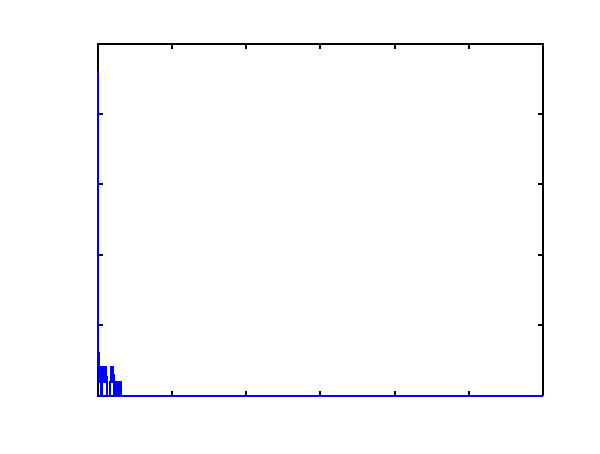
\includegraphics{plot/q15-inc}
\end{picture}%
\begin{picture}(288,218)(0,0)
\fontsize{10}{0}
\selectfont\put(47.0044,22.9956){\makebox(0,0)[t]{\textcolor[rgb]{0,0,0}{{0}}}}
\fontsize{10}{0}
\selectfont\put(82.6104,22.9956){\makebox(0,0)[t]{\textcolor[rgb]{0,0,0}{{5000}}}}
\fontsize{10}{0}
\selectfont\put(118.216,22.9956){\makebox(0,0)[t]{\textcolor[rgb]{0,0,0}{{10000}}}}
\fontsize{10}{0}
\selectfont\put(153.822,22.9956){\makebox(0,0)[t]{\textcolor[rgb]{0,0,0}{{15000}}}}
\fontsize{10}{0}
\selectfont\put(189.428,22.9956){\makebox(0,0)[t]{\textcolor[rgb]{0,0,0}{{20000}}}}
\fontsize{10}{0}
\selectfont\put(225.034,22.9956){\makebox(0,0)[t]{\textcolor[rgb]{0,0,0}{{25000}}}}
\fontsize{10}{0}
\selectfont\put(260.64,22.9956){\makebox(0,0)[t]{\textcolor[rgb]{0,0,0}{{30000}}}}
\fontsize{10}{0}
\selectfont\put(42.0132,27.9961){\makebox(0,0)[r]{\textcolor[rgb]{0,0,0}{{0.1}}}}
\fontsize{10}{0}
\selectfont\put(42.0132,61.7969){\makebox(0,0)[r]{\textcolor[rgb]{0,0,0}{{0.15}}}}
\fontsize{10}{0}
\selectfont\put(42.0132,95.5977){\makebox(0,0)[r]{\textcolor[rgb]{0,0,0}{{0.2}}}}
\fontsize{10}{0}
\selectfont\put(42.0132,129.398){\makebox(0,0)[r]{\textcolor[rgb]{0,0,0}{{0.25}}}}
\fontsize{10}{0}
\selectfont\put(42.0132,163.199){\makebox(0,0)[r]{\textcolor[rgb]{0,0,0}{{0.3}}}}
\fontsize{10}{0}
\selectfont\put(42.0132,197){\makebox(0,0)[r]{\textcolor[rgb]{0,0,0}{{0.35}}}}
\fontsize{10}{0}
\selectfont\put(153.822,11.9956){\makebox(0,0)[t]{\textcolor[rgb]{0,0,0}{{t}}}}
\fontsize{10}{0}
\selectfont\put(17.0132,112.498){\rotatebox{90}{\makebox(0,0)[b]{\textcolor[rgb]{0,0,0}{{$E_{in}(G_t)$}}}}}
\fontsize{10}{0}
\selectfont\put(153.822,207){\makebox(0,0)[b]{\textcolor[rgb]{0,0,0}{{Result of Question 15}}}}
\end{picture}

  \item The relation between $t$ and $E_\text{out}(G_t)$ is shown below. Similar with Questions 13-14, both $E_\text{in}$ and $E_\text{out}$ will approach a constant when $t$ is large: $E_\text{in}$ will end up with 0.1, while $E_\text{out}$ will end up with 0.145 (small difference may occur).\\
  \begin{picture}(0,0)
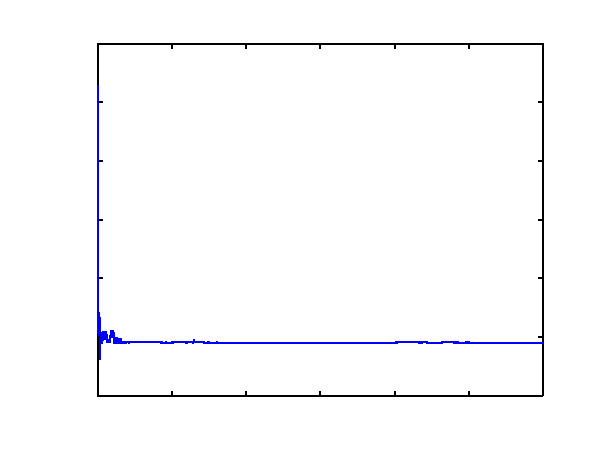
\includegraphics{plot/q16-inc}
\end{picture}%
\begin{picture}(288,218)(0,0)
\fontsize{10}{0}
\selectfont\put(47.0044,22.9956){\makebox(0,0)[t]{\textcolor[rgb]{0,0,0}{{0}}}}
\fontsize{10}{0}
\selectfont\put(82.6104,22.9956){\makebox(0,0)[t]{\textcolor[rgb]{0,0,0}{{5000}}}}
\fontsize{10}{0}
\selectfont\put(118.216,22.9956){\makebox(0,0)[t]{\textcolor[rgb]{0,0,0}{{10000}}}}
\fontsize{10}{0}
\selectfont\put(153.822,22.9956){\makebox(0,0)[t]{\textcolor[rgb]{0,0,0}{{15000}}}}
\fontsize{10}{0}
\selectfont\put(189.428,22.9956){\makebox(0,0)[t]{\textcolor[rgb]{0,0,0}{{20000}}}}
\fontsize{10}{0}
\selectfont\put(225.034,22.9956){\makebox(0,0)[t]{\textcolor[rgb]{0,0,0}{{25000}}}}
\fontsize{10}{0}
\selectfont\put(260.64,22.9956){\makebox(0,0)[t]{\textcolor[rgb]{0,0,0}{{30000}}}}
\fontsize{10}{0}
\selectfont\put(42.0132,27.9961){\makebox(0,0)[r]{\textcolor[rgb]{0,0,0}{{0.1}}}}
\fontsize{10}{0}
\selectfont\put(42.0132,56.1631){\makebox(0,0)[r]{\textcolor[rgb]{0,0,0}{{0.15}}}}
\fontsize{10}{0}
\selectfont\put(42.0132,84.3306){\makebox(0,0)[r]{\textcolor[rgb]{0,0,0}{{0.2}}}}
\fontsize{10}{0}
\selectfont\put(42.0132,112.498){\makebox(0,0)[r]{\textcolor[rgb]{0,0,0}{{0.25}}}}
\fontsize{10}{0}
\selectfont\put(42.0132,140.666){\makebox(0,0)[r]{\textcolor[rgb]{0,0,0}{{0.3}}}}
\fontsize{10}{0}
\selectfont\put(42.0132,168.833){\makebox(0,0)[r]{\textcolor[rgb]{0,0,0}{{0.35}}}}
\fontsize{10}{0}
\selectfont\put(42.0132,197){\makebox(0,0)[r]{\textcolor[rgb]{0,0,0}{{0.4}}}}
\fontsize{10}{0}
\selectfont\put(153.822,11.9956){\makebox(0,0)[t]{\textcolor[rgb]{0,0,0}{{t}}}}
\fontsize{10}{0}
\selectfont\put(17.0132,112.498){\rotatebox{90}{\makebox(0,0)[b]{\textcolor[rgb]{0,0,0}{{$E_{out}(G_t)$}}}}}
\fontsize{10}{0}
\selectfont\put(153.822,207){\makebox(0,0)[b]{\textcolor[rgb]{0,0,0}{{Result of Question 16}}}}
\end{picture}


\end{enumerate}

\end{document}
